\chapter{Results}

\section{Data}
Data was obtained through the \gls{CDD} for different \glspl{MSA} from the list of 49 selected in the \textit{E}-score paper (\cite{Marchler-Bauer:2015, Ashrafzadeh:2023}). Selected \glspl{MSA} are found in Table \ref{tab:msa} and in the \href{https://github.com/rgavigan/e-score/tree/bf08fa86209a6ce9956d48212690b1814450e72b/data/finetuning/msa-proteins}{code repository}.

\begin{table*} % Two column table
	\caption{10 MSAs with the most proteins from CDD used in the \textit{E}-score comparison procedure (\cite{Ashrafzadeh:2023, Marchler-Bauer:2015}).}
	\centering
    \vspace{2mm}
    \scalebox{0.9}{
	\begin{tabular}{ lrrr }
		\toprule
        \multicolumn{4}{c}{MSAs} \\
        \midrule
		Conserved Domain & Source & Proteins & Length \\
		\midrule
        \(CS\_CSD\) & cd00024 & 522 & 98 \\
        \(7tm\_classA\_rhodopsin\-like\) & cd00637 & 405 & 808 \\
        \(FYVE\_like\_SF\) & cd00065 & 392 & 266 \\
        \(Mb\-like\) & cd01040 & 384 & 239 \\
        \(SH2\) & cd00173 & 352 & 214 \\
        \(C1\) & cd00029 & 281 & 99 \\
        \(KAZAL\_FS\) & cd00104 & 273 & 74 \\
        \(Globin\_sensor\) & cd01068 & 193 & 223 \\
        \(Bbox2\) & cd19756 & 127 & 65 \\
        \(NBD\_sugar\-kinase\_HSP70\_actin\) & cd00012 & 125 & 1154 \\
		\bottomrule
	\end{tabular}
    }
	\label{tab:msa}
\end{table*}

\noindent Procedure for obtaining CDD MSA data:
\begin{enumerate}
    \item{Select a source from Table \ref{tab:msa}.}
    \item{Search for the source on the \href{https://www.ncbi.nlm.nih.gov/cdd}{CDD website}.}
    \item{Click 'Representatives' under 'Links', send to FASTA format.}
    \item{For reference alignments: click 'Download Alignment' instead of going to 'Representatives'}
\end{enumerate}

\noindent Alignment pairs \(i, j\) were enumerated by iterating through each FASTA file: \(\forall i~\forall j, ~i \ne j\). These pairs were used to determine embedding value distributions (\hyperlink{O1}{O1}) and cosine similarity distributions (\hyperlink{O3}{O3})  for natural proteins. Reference alignments serve as necessary data for future fine-tuning efforts based on drawn conclusions.

Random sequence data was generated by randomly selecting \glspl{residue} of equal probability with replacement for sequences of random lengths between 100 and 400. This data was used to compare random embeddings and cosine similarity to naturally-observed results (\hyperlink{O1}{O1}).

\section{Protein composition}

Sequence similarity is essential in sequence analysis within bioinformatics (\cite{Ofer:2021}). Peptide sequence alignment is the most complex case, with a language of 20 common \glspl{amino acids} forming a theoretically countably infinite amount of unique \gls{peptide} sequences shown in Equation \ref{eq:peptideinfinity} by taking the n-ary Cartesian product.

\begin{equation}
    {Theoretical\, Limit} = \prod_{k=1}^{\infty} |A| = \prod_{k=1}^{\infty} 20 = 20 \times 20 \times \ldots
    \label{eq:peptideinfinity}
\end{equation}

Observed sequences in living organisms are constrained by biological, genetic, and functional factors. For example, the average eukaryotic protein size is $353 \pm 62.5$ \glspl{residue} (\cite{Nevers:2023}). 

Databases such as UniProt (\cite{UniProt:2023}) and PeptideAtlas (\cite{PeptideAtlas:2006}) are repositories filled with \gls{peptide} sequences. UniProt contains over 250 million unique peptide sequences and counting (\cite{UniProt:2023}).

Peptide sequences are not completely random because of the constraints imposed on them. Similar to letters or words in a given language within natural language, the frequency of each \gls{amino acids} observed in nature is not equally distributed (\cite{Beals:1999}).

Proteins form secondary structures as part of larger tertiary and quaternary structures. The most common of these secondary structures are \(\alpha\) helices and \(\beta\) pleated sheets (\cite{Ma:2018}). Because of this, algorithms such as an \gls{ENNA} are able to distinguish natural proteins from randomly generated proteins with an accuracy of over 94\% (\cite{Lucrezia:2012}).

The distribution of the observed amino acids in all of the protein sequences from the 10 MSAs in Table \ref{tab:msa} is shown in Table \ref{tab:aadist}. Counts were acquired by reading FASTA file sequences for each MSA and generating a \LaTeX~table containing names, frequencies, and percentages for the 20 most common \glspl{amino acids}.

\begin{table}[H] % Two column table
	\caption{Distribution of amino acids found in the 10 selected MSAs. A few occurrences of 'B' (nondeterministically either N or D) and some occurrences of 'X' (undetermined or atypical amino acid) were left out for simplicity.}
	\centering
    \vspace{2mm}
    \begin{tabular}{lrrrrl}
    \toprule
     Amino Acid & Symbol & Frequency & Percent & Diff From Equal & P-value \\
    \midrule
    Leucine & L & 152859 & 9.099 & 4.099 & 0.0e+00 \\
    Serine & S & 141844 & 8.443 & 3.443 & 0.0e+00 \\
    Alanine & A & 127926 & 7.614 & 2.614 & 0.0e+00 \\
    Glutamic Acid & E & 108476 & 6.457 & 1.457 & 0.0e+00 \\
    Valine & V & 105408 & 6.274 & 1.274 & 0.0e+00 \\
    Arginine & R & 99687 & 5.934 & 0.934 & 3.2e-293 \\
    Glycine & G & 96906 & 5.768 & 0.768 & 3.6e-202 \\
    Threonine & T & 96702 & 5.756 & 0.756 & 4.1e-196 \\
    Lysine & K & 94251 & 5.610 & 0.610 & 3.6e-130 \\
    Aspartic Acid & D & 88980 & 5.296 & 0.296 & 5.2e-33 \\
    Isoleucine & I & 87579 & 5.213 & 0.213 & 5.9e-18 \\
    Proline & P & 86463 & 5.146 & 0.146 & 2.5e-09 \\
    Glutamine & Q & 74206 & 4.417 & 0.583 & 6.3e-134 \\
    Asparagine & N & 73490 & 4.374 & 0.626 & 1.3e-154 \\
    Phenylalanine & F & 64495 & 3.839 & 1.161 & 0.0e+00 \\
    Tyrosine & Y & 46324 & 2.757 & 2.243 & 0.0e+00 \\
    Histidine & H & 43163 & 2.569 & 2.431 & 0.0e+00 \\
    Cysteine & C & 36749 & 2.187 & 2.813 & 0.0e+00 \\
    Methionine & M & 35289 & 2.100 & 2.900 & 0.0e+00 \\
    Tryptophan & W & 19243 & 1.145 & 3.855 & 0.0e+00 \\
    \bottomrule
    \end{tabular}
	\label{tab:aadist}
\end{table}

\section{\textit{E}-score model differences}
The \gls{transformer} models used in the \textit{E}-score method (see Table \ref{tab:transformers}) vary in performance (\hyperlink{O1}{O1}). ProtT5 outperformed the 5 other models available when computing end-gap-free alignments for six different conserved domain \glspl{MSA}. ProtT5 and ESM2, the second best model, were compared and it was evident that ProtT5 outperformed ESM2 with statistically significant results (\cite{Ashrafzadeh:2023}).

\textit{E}-score's protein transformers models have significantly different pre-training configurations (\cite{Elnaggar:2021, Rives:2021}), some of which are highlighted in Table \ref{tab:prottrans} (\hyperlink{O1}{O1}).

\begin{table*} % Two column table
	\caption{Pre-training configuration for protein language models (\cite{Elnaggar:2021,Rives:2021}). UR = UniRef.}
	\centering
	\begin{tabular}{ lllllll }
		\toprule
		Hyperparam & ProtT5 & ProtBert & ProtXLNet & ProtAlbert & ESM1b & ESM2 \\
		\midrule
		Dataset & UR50 & UR100 & UR100 & UR100 & UR50 & UR50 \\
		\# of Layers & 24 & 30 & 30 & 12 & 33 & 33 \\
		Embedding Dim & 1024 & 1024 & 1024 & 4096 & 1280 & 1280 \\
        \# of Params & 3B & 420M & 409M & 224M & 650M & 650M \\
        Learning Rate & 0.01 & 0.002 & 0.00001 & 0.002 & 0.0004 & 0.0004 \\
		\bottomrule
	\end{tabular}
	\label{tab:prottrans}
\end{table*}

Protein transformer model pre-training configurations significantly impact model performance. For example, ProtT5 has 3 billion parameters compared to ProtAlbert having 224 million. Model performance and number of parameters are highly correlated, which is supported by the Chinchilla paper's findings for training compute-optimal \glspl{LLM} (\cite{Hoffman:2022}). Through the results from the comparison between models in the \textit{E}-score paper (\cite{Ashrafzadeh:2023}), it was evident that the encoder-decoder model ProtT5 outperformed both the encoder-only models (ESM1b, ESM2, ProtBert, ProtAlbert) and the decoder-only model (XLNet).

\section{Embeddings}
Understanding embedding distributions is crucial in understanding cosine similarity results and how they can be improved (\hyperlink{O2}{O2}). Embedding distributions were compared for all ProtTrans models in the \textit{E}-score method for both randomly selected natural protein sequences and randomly generated sequences. Embedding value distributions are visualized in Figure \ref{fig:embedding_avg}.     The procedure for obtaining average embedding values is described below:
\begin{itemize}
    \item{Obtain n sequences to provide as input to a model}
    \item{Produce and store the embedding values for all n sequences}
    \item{Normalize the embedding values, then obtain the average and standard deviation of all n embeddings}
\end{itemize}

\begin{figure}[H]
    \begin{center}
	   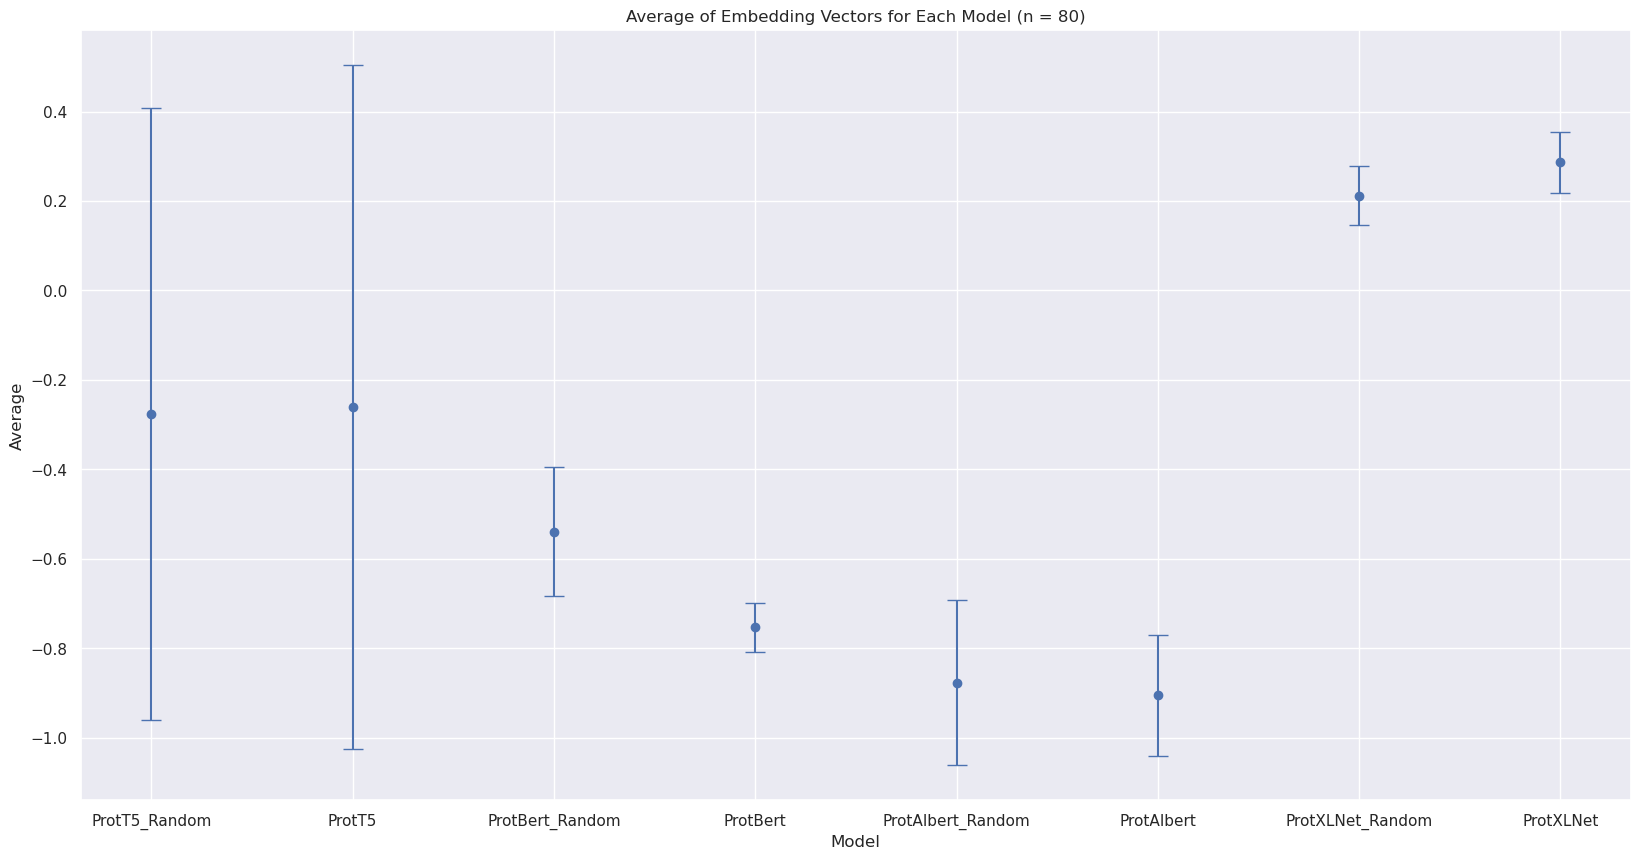
\includegraphics[width=0.9\linewidth]{figures/embedding_avg.png}
    \end{center}
    \caption{Average embedding values for 80 random and non-random (randomly chosen from CDD) embeddings for all ProtTrans models. Values scaled to -1...1.}
    \label{fig:embedding_avg}
\end{figure}

\section{Cosine Similarity}
Cosine similarity distributions were compared for all ProtTrans models in the \textit{E}-score method for randomly selected natural protein sequences and randomly generated sequences. Cosine similarity distributions are visualized in Figure \ref{fig:random_vs_nonrandom_cossim}. The procedure for determining cosine similarity distributions is described below:
\begin{itemize}
    \item{Get embeddings for n sequences from a selected model.}
    \item{Calculate the cosine similarity between every pair \(i, j\) of embeddings, for a total of \(n^2\) cosine similarity calculations.}
\end{itemize}


\begin{figure}[H]
    \begin{center}
	   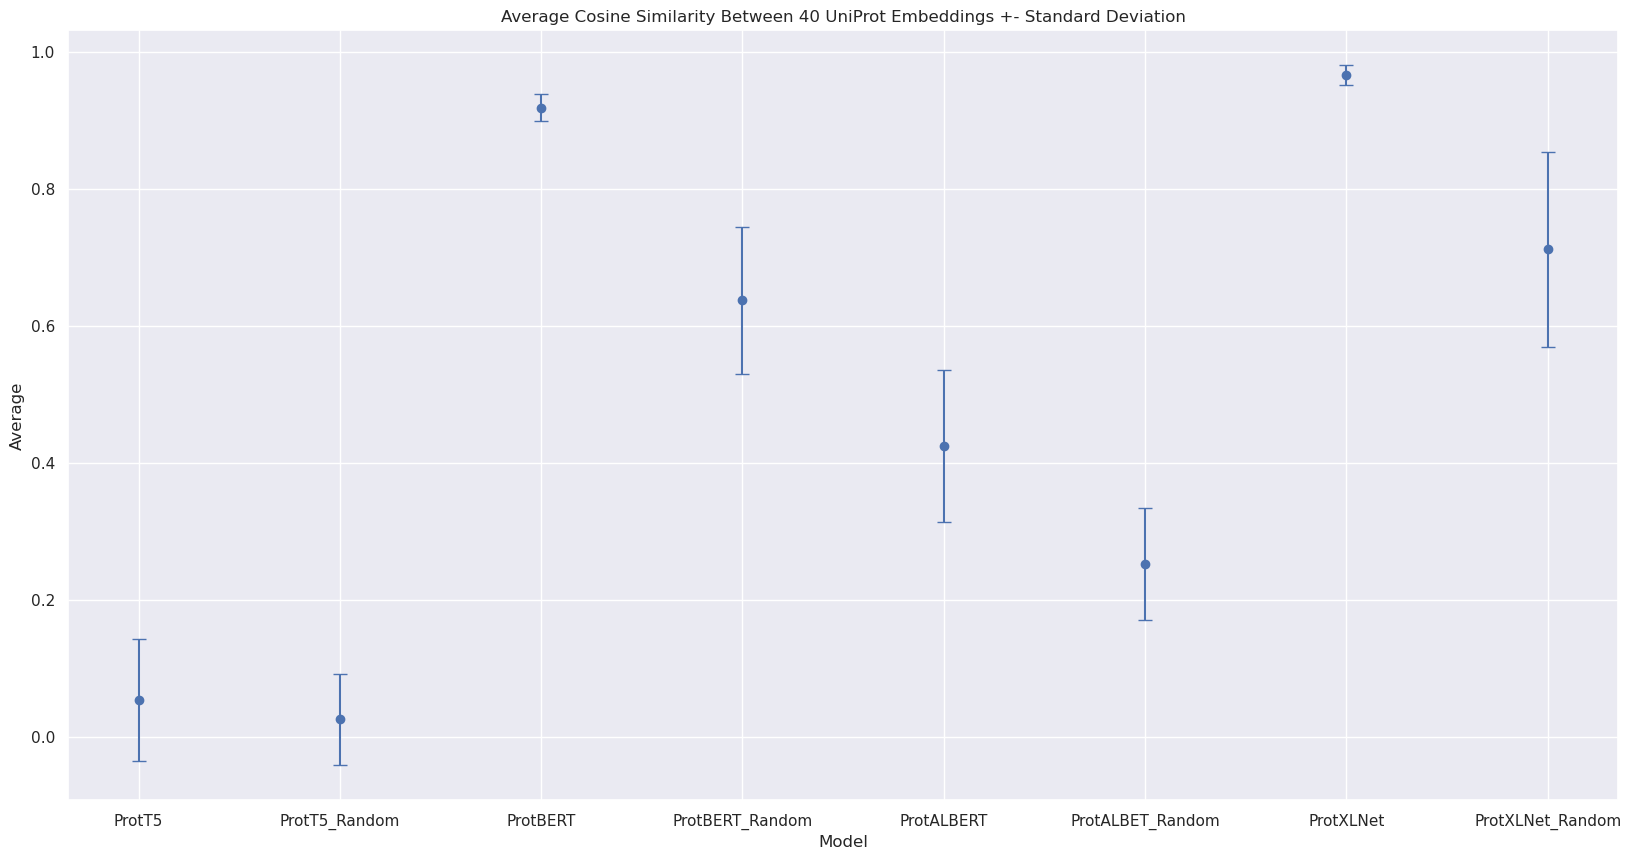
\includegraphics[width=1.0\linewidth]{figures/random_vs_nonrandom_cossim.png}
    \end{center}
    \caption{Average cosine similarity between sample and random embeddings for all ProtTrans models. P-Values are all \(0.000\) between any column and overall average of 0.59 (and between any chosen comparison).}
    \label{fig:random_vs_nonrandom_cossim}
\end{figure}
